\chapter{計算機実験}
\label{chp:fourth}
本章では，先行研究を再現した配置Iと，本研究で説明した合成駒を用いた配置IIの比較とそれぞれの手数についての結果を，
様々な入力例を用いて示す．配置IIでは，空所となる位置を，パリティ判定を用いて（\ref{fig:thm1}）決定した．
また，手数については\ref{sec:greed}の「距離コストの計算を用いた行（列）の選択」を前者では使用せず，
後者では使用する，という違いのみで計算した値を使用する．
実験では，$n=20$，$n=30$，$n=50$の場合にわけて実験を行う．
以下（図\ref{fig:ex1}〜図\ref{fig:ex10}）は，本章で用いる入力画像である．
\begin{figure}[H]
	\centering
	\begin{minipage}[t]{0.3\hsize}
		\centering
		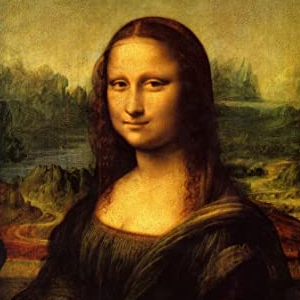
\includegraphics[width=4cm]{./fig/1.png}
		\caption{入力例1}
		\label{fig:ex1}
	\end{minipage}
	\begin{minipage}[t]{0.3\hsize}
		\centering
		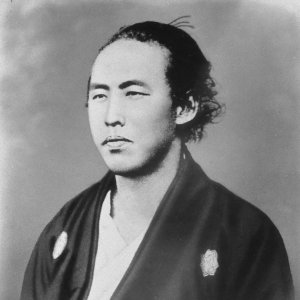
\includegraphics[width=4cm]{./fig/2.png}
		\caption{入力例2}
		\label{fig:ex2}
    \end{minipage}
    \begin{minipage}[t]{0.3\hsize}
		\centering
		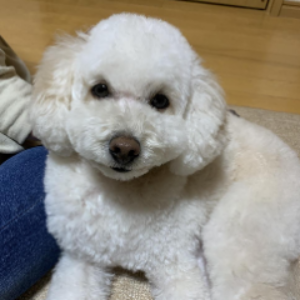
\includegraphics[width=4cm]{./fig/3.png}
		\caption{入力例3}
		\label{fig:ex3}
	\end{minipage}
	% \url{http://www.this.is.sample.url/} % Web上のデータの場合、参照先URLを明記
\end{figure}
\begin{figure}[H]
	\centering
	\begin{minipage}[t]{0.3\hsize}
		\centering
		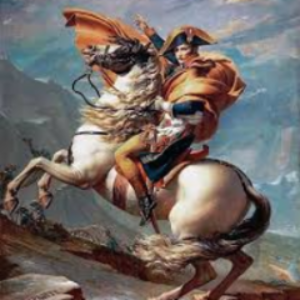
\includegraphics[width=4cm]{./fig/4.png}
		\caption{入力例4}
		\label{fig:ex4}
    \end{minipage}
    \begin{minipage}[t]{0.3\hsize}
		\centering
		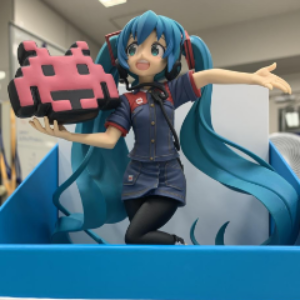
\includegraphics[width=4cm]{./fig/5.png}
		\caption{入力例5}
		\label{fig:ex5}
    \end{minipage}
    \begin{minipage}[t]{0.3\hsize}
		\centering
		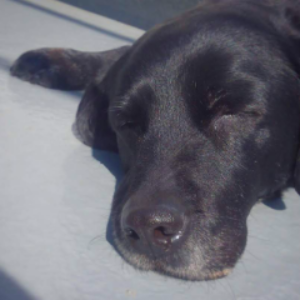
\includegraphics[width=4cm]{./fig/6.png}
		\caption{入力例6}
		\label{fig:ex6}
	\end{minipage}
	% \url{http://www.this.is.sample.url/} % Web上のデータの場合、参照先URLを明記
\end{figure}
\begin{figure}[H]
	\centering
	\begin{minipage}[t]{0.3\hsize}
		\centering
		
\includegraphics[width=4cm]{./fig/7.png}
		\caption{入力例7}
		\label{fig:ex7}
    \end{minipage}
    \begin{minipage}[t]{0.3\hsize}
		\centering
		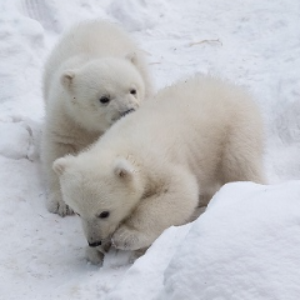
\includegraphics[width=4cm]{./fig/8.png}
		\caption{入力例8}
		\label{fig:ex8}
    \end{minipage}
    \begin{minipage}[t]{0.3\hsize}
		\centering
		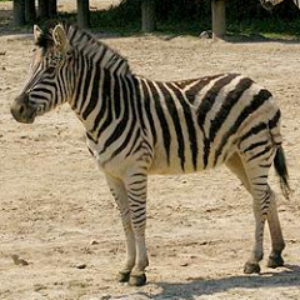
\includegraphics[width=4cm]{./fig/9.png}
		\caption{入力例9}
		\label{fig:ex9}
	\end{minipage}
	% \url{http://www.this.is.sample.url/} % Web上のデータの場合、参照先URLを明記
\end{figure}
\begin{figure}[H]
	\centering
	\begin{minipage}[t]{0.3\hsize}
		\centering
		
\includegraphics[width=4cm]{./fig/10.png}
		\caption{入力例10}
		\label{fig:ex10}
    \end{minipage}
	% \url{http://www.this.is.sample.url/} % Web上のデータの場合、参照先URLを明記
\end{figure}
\newpage
\section{配置と手数の比較}
\textbf{入力例1と入力例2}

\textbf{n=20}
\begin{figure}[H]
	\centering
	\begin{minipage}[t]{0.3\hsize}
		\centering
		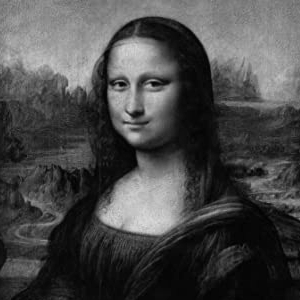
\includegraphics[width=4cm]{./fig/g1.png}
		\caption{入力例1(グレー)}
		\label{fig:exg1}
	\end{minipage}
	\begin{minipage}[t]{0.3\hsize}
		\centering
		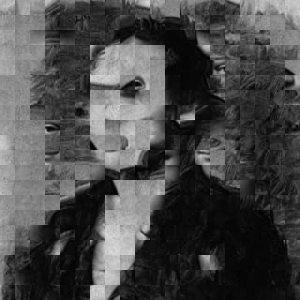
\includegraphics[width=4cm]{./fig/pre2_20.png}
		\caption{入力例2(配置I)}
		\label{fig:p2_20}
    \end{minipage}
    
	% \url{http://www.this.is.sample.url/} % Web上のデータの場合、参照先URLを明記
\end{figure}
\begin{figure}[H]
	\centering
	\begin{minipage}[t]{0.3\hsize}
		\centering
		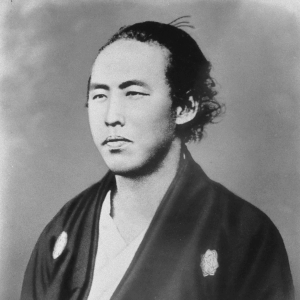
\includegraphics[width=4cm]{./fig/g2.png}
		\caption{入力例2(グレー)}
		\label{fig:exg2}
    \end{minipage}
	\begin{minipage}[t]{0.3\hsize}
		\centering
		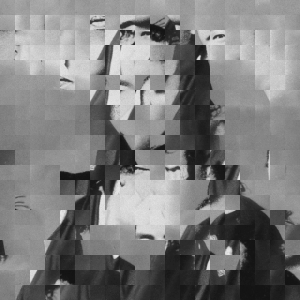
\includegraphics[width=4cm]{./fig/pre1_20.png}
        \caption{入力例1(配置I)}
		\label{fig:p1_20}
    \end{minipage}
    
	% \url{http://www.this.is.sample.url/} % Web上のデータの場合、参照先URLを明記
\end{figure}
\begin{figure}[H]
	\centering
	\begin{minipage}[t]{0.3\hsize}
		\centering
		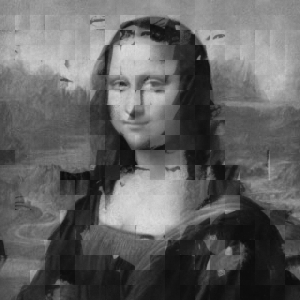
\includegraphics[width=4cm]{./fig/main1_20.png}
        \caption{入力例1(配置II)}
		\label{fig:m1_2_20}
    \end{minipage}
    \begin{minipage}[t]{0.3\hsize}
		\centering
		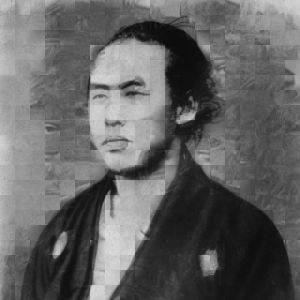
\includegraphics[width=4cm]{./fig/main2_20.png}
		\caption{入力例2(配置II)}
		\label{fig:m2_20}
    \end{minipage}
	% \url{http://www.this.is.sample.url/} % Web上のデータの場合、参照先URLを明記
\end{figure}
\newpage
\textbf{n=30}
\begin{figure}[H]
	\centering
	\begin{minipage}[t]{0.3\hsize}
		\centering
		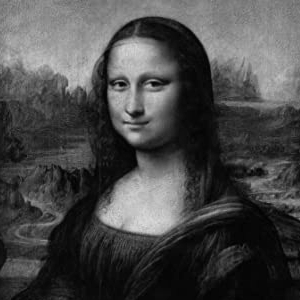
\includegraphics[width=4cm]{./fig/g1.png}
		\caption{入力例1(グレー)}
		\label{fig:exg1}
	\end{minipage}
	\begin{minipage}[t]{0.3\hsize}
		\centering
		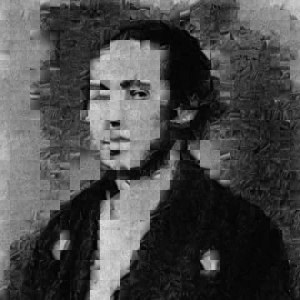
\includegraphics[width=4cm]{./fig/pre2_30.png}
		\caption{入力例2(配置I)}
		\label{fig:p2_30}
    \end{minipage}
    
	% \url{http://www.this.is.sample.url/} % Web上のデータの場合、参照先URLを明記
\end{figure}
\begin{figure}[H]
	\centering
	\begin{minipage}[t]{0.3\hsize}
		\centering
		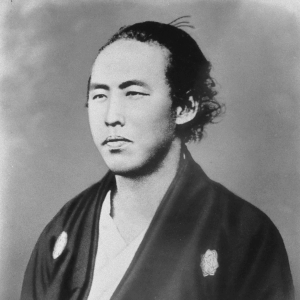
\includegraphics[width=4cm]{./fig/g2.png}
		\caption{入力例2(グレー)}
		\label{fig:exg2}
    \end{minipage}
	\begin{minipage}[t]{0.3\hsize}
		\centering
		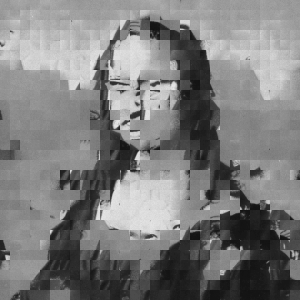
\includegraphics[width=4cm]{./fig/pre1_30.png}
        \caption{入力例1(配置I)}
		\label{fig:p1_30}
    \end{minipage}
	% \url{http://www.this.is.sample.url/} % Web上のデータの場合、参照先URLを明記
\end{figure}
\begin{figure}[H]
	\centering
	\begin{minipage}[t]{0.3\hsize}
		\centering
		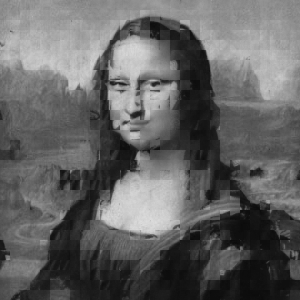
\includegraphics[width=4cm]{./fig/main1_30.png}
        \caption{入力例1(配置II)}
		\label{fig:m1_2_30}
    \end{minipage}
    \begin{minipage}[t]{0.3\hsize}
		\centering
		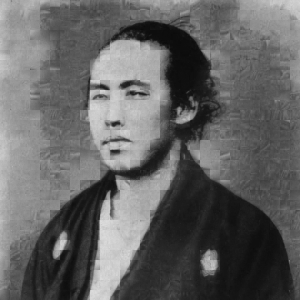
\includegraphics[width=4cm]{./fig/main2_30.png}
		\caption{入力例2(配置II)}
		\label{fig:m2_30}
    \end{minipage}
	% \url{http://www.this.is.sample.url/} % Web上のデータの場合、参照先URLを明記
\end{figure}
\newpage
\textbf{n=50}
\begin{figure}[H]
	\centering
	\begin{minipage}[t]{0.3\hsize}
		\centering
		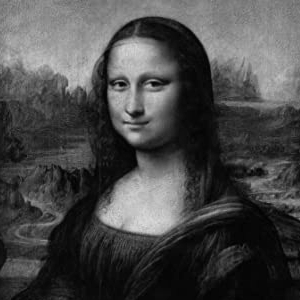
\includegraphics[width=4cm]{./fig/g1.png}
		\caption{入力例1(グレー)}
		\label{fig:exg1}
	\end{minipage}
	\begin{minipage}[t]{0.3\hsize}
		\centering
		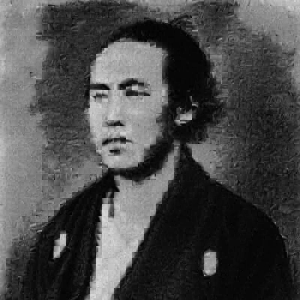
\includegraphics[width=4cm]{./fig/pre2_50.png}
		\caption{入力例2(配置I)}
		\label{fig:p2_50}
    \end{minipage}
    
	% \url{http://www.this.is.sample.url/} % Web上のデータの場合、参照先URLを明記
\end{figure}
\begin{figure}[H]
	\centering
	\begin{minipage}[t]{0.3\hsize}
		\centering
		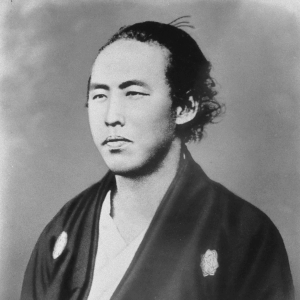
\includegraphics[width=4cm]{./fig/g2.png}
		\caption{入力例2(グレー)}
		\label{fig:exg2}
    \end{minipage}
	\begin{minipage}[t]{0.3\hsize}
		\centering
		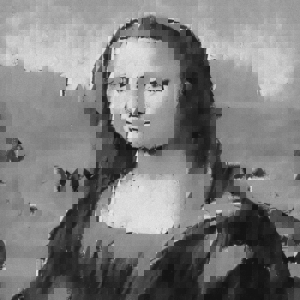
\includegraphics[width=4cm]{./fig/pre1_50.png}
        \caption{入力例1(配置I)}
		\label{fig:p1_50}
    \end{minipage}
	% \url{http://www.this.is.sample.url/} % Web上のデータの場合、参照先URLを明記
\end{figure}
\begin{figure}[H]
	\centering
	\begin{minipage}[t]{0.3\hsize}
		\centering
		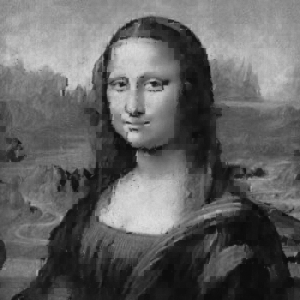
\includegraphics[width=4cm]{./fig/main1_50.png}
        \caption{入力例1(配置II)}
		\label{fig:m1_2_50}
    \end{minipage}
    \begin{minipage}[t]{0.3\hsize}
		\centering
		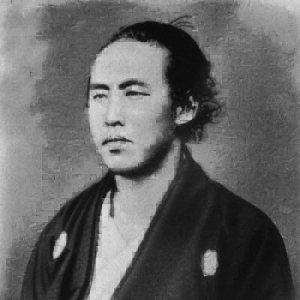
\includegraphics[width=4cm]{./fig/main2_50.png}
		\caption{入力例2(配置II)}
		\label{fig:m2_50}
    \end{minipage}
	% \url{http://www.this.is.sample.url/} % Web上のデータの場合、参照先URLを明記
\end{figure}
\begin{table}[H]
    \centering
    \caption{入力例1($\ref{fig:exg1}$)と入力例2($\ref{fig:exg2}$)での完成手数}
    \begin{tabular}{|c|c|c|c|} \hline
    　 & $n=20$ & $n=30$ & $n=50$ \\ \hline
    先行研究（再現） & 19,644 & 66,103 & 311,535 \\ \hline
    本研究 & 18,848 & 66,037 & 311,391 \\ \hline
    \end{tabular}
    \label{tab:1_2pzl}
\end{table}
\newpage
\textbf{入力例6と入力例7}

\textbf{n=20}
\begin{figure}[H]
	\centering
	\begin{minipage}[t]{0.3\hsize}
		\centering
		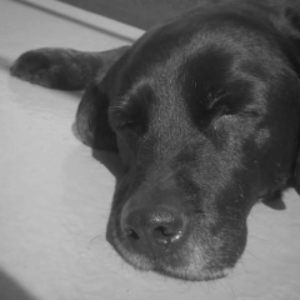
\includegraphics[width=4cm]{./fig/g6.png}
		\caption{入力例6(グレー)}
		\label{fig:exg6}
	\end{minipage}
	\begin{minipage}[t]{0.3\hsize}
		\centering
		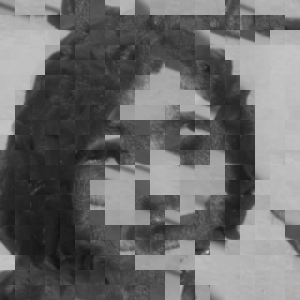
\includegraphics[width=4cm]{./fig/pre7_20.png}
		\caption{入力例7(配置I)}
		\label{fig:p7_20}
    \end{minipage}
	% \url{http://www.this.is.sample.url/} % Web上のデータの場合、参照先URLを明記
\end{figure}
\begin{figure}[H]
	\centering
	\begin{minipage}[t]{0.3\hsize}
		\centering
		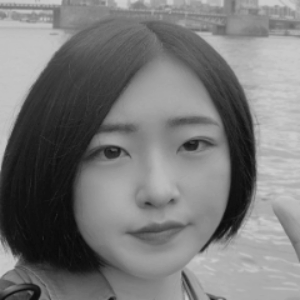
\includegraphics[width=4cm]{./fig/g7.png}
		\caption{入力例7(グレー)}
		\label{fig:exg7}
    \end{minipage}
	\begin{minipage}[t]{0.3\hsize}
		\centering
		
\includegraphics[width=4cm]{./fig/pre6_20.png}
        \caption{入力例6(配置I)}
		\label{fig:p6_20}
    \end{minipage}
	% \url{http://www.this.is.sample.url/} % Web上のデータの場合、参照先URLを明記
\end{figure}
\begin{figure}[H]
	\centering
	\begin{minipage}[t]{0.3\hsize}
		\centering
		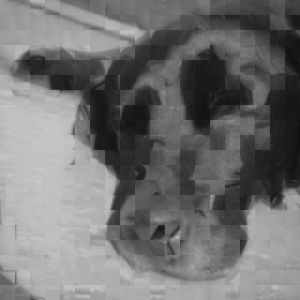
\includegraphics[width=4cm]{./fig/main6_20.png}
        \caption{入力例6(配置II)}
		\label{fig:m6_20}
    \end{minipage}
    \begin{minipage}[t]{0.3\hsize}
		\centering
		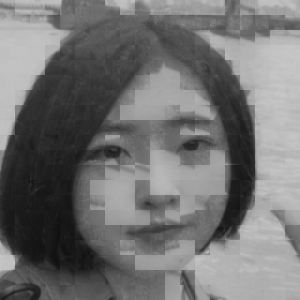
\includegraphics[width=4cm]{./fig/main7_20.png}
		\caption{入力例7(配置II)}
		\label{fig:m7_20}
    \end{minipage}
	% \url{http://www.this.is.sample.url/} % Web上のデータの場合、参照先URLを明記
\end{figure}
\newpage
\textbf{n=30}
\begin{figure}[H]
	\centering
	\begin{minipage}[t]{0.3\hsize}
		\centering
		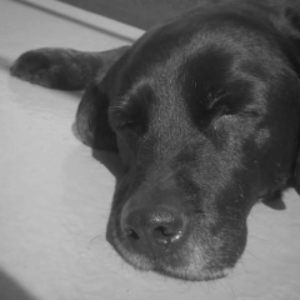
\includegraphics[width=4cm]{./fig/g6.png}
		\caption{入力例6(グレー)}
		\label{fig:exg6}
	\end{minipage}
	\begin{minipage}[t]{0.3\hsize}
		\centering
		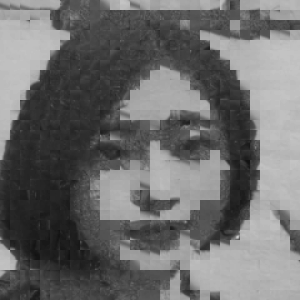
\includegraphics[width=4cm]{./fig/pre7_30.png}
		\caption{入力例7(配置I)}
		\label{fig:p7_30}
    \end{minipage}
	% \url{http://www.this.is.sample.url/} % Web上のデータの場合、参照先URLを明記
\end{figure}
\begin{figure}[H]
	\centering
	\begin{minipage}[t]{0.3\hsize}
		\centering
		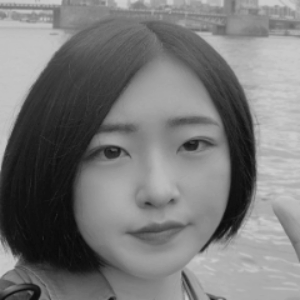
\includegraphics[width=4cm]{./fig/g7.png}
		\caption{入力例7(グレー)}
		\label{fig:exg7}
    \end{minipage}
	\begin{minipage}[t]{0.3\hsize}
		\centering
		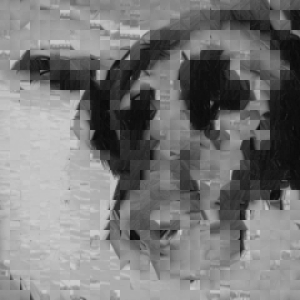
\includegraphics[width=4cm]{./fig/pre6_30.png}
        \caption{入力例6(配置I)}
		\label{fig:p6_30}
    \end{minipage}
	% \url{http://www.this.is.sample.url/} % Web上のデータの場合、参照先URLを明記
\end{figure}
\begin{figure}[H]
	\centering
	\begin{minipage}[t]{0.3\hsize}
		\centering
		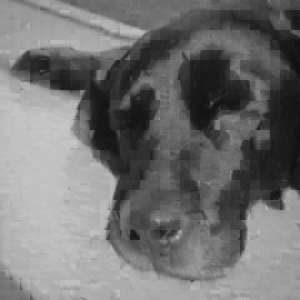
\includegraphics[width=4cm]{./fig/main6_30.png}
        \caption{入力例6(配置II)}
		\label{fig:m6_30}
    \end{minipage}
    \begin{minipage}[t]{0.3\hsize}
		\centering
		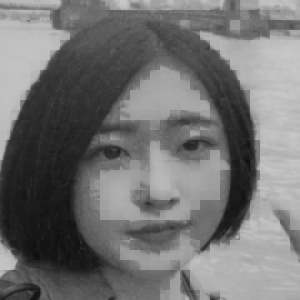
\includegraphics[width=4cm]{./fig/main7_30.png}
		\caption{入力例7(配置II)}
		\label{fig:m7_30}
    \end{minipage}
	% \url{http://www.this.is.sample.url/} % Web上のデータの場合、参照先URLを明記
\end{figure}
\newpage
\textbf{n=50}
\begin{figure}[H]
	\centering
	\begin{minipage}[t]{0.3\hsize}
		\centering
		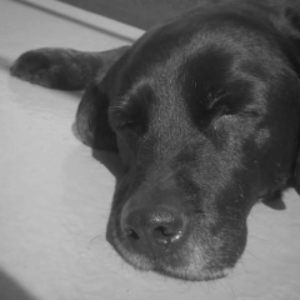
\includegraphics[width=4cm]{./fig/g6.png}
		\caption{入力例6(グレー)}
		\label{fig:exg6}
	\end{minipage}
	\begin{minipage}[t]{0.3\hsize}
		\centering
		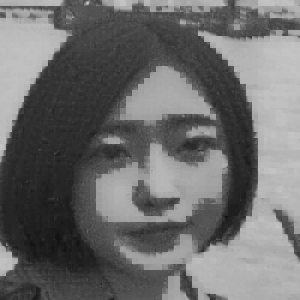
\includegraphics[width=4cm]{./fig/pre7_50.png}
		\caption{入力例7(配置I)}
		\label{fig:p7_50}
    \end{minipage}
	% \url{http://www.this.is.sample.url/} % Web上のデータの場合、参照先URLを明記
\end{figure}
\begin{figure}[H]
	\centering
	\begin{minipage}[t]{0.3\hsize}
		\centering
		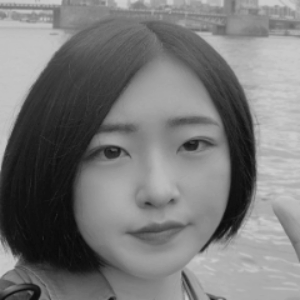
\includegraphics[width=4cm]{./fig/g7.png}
		\caption{入力例7(グレー)}
		\label{fig:exg7}
    \end{minipage}
	\begin{minipage}[t]{0.3\hsize}
		\centering
		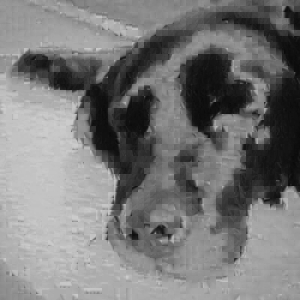
\includegraphics[width=4cm]{./fig/pre6_50.png}
        \caption{入力例6(配置I)}
		\label{fig:p6_50}
    \end{minipage}
	% \url{http://www.this.is.sample.url/} % Web上のデータの場合、参照先URLを明記
\end{figure}
\begin{figure}[H]
	\centering
	\begin{minipage}[t]{0.3\hsize}
		\centering
		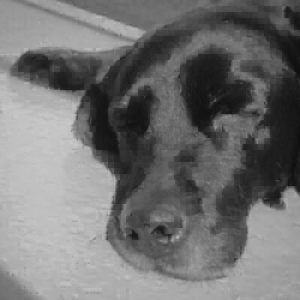
\includegraphics[width=4cm]{./fig/main6_50.png}
        \caption{入力例6(配置II)}
		\label{fig:m6_50}
    \end{minipage}
    \begin{minipage}[t]{0.3\hsize}
		\centering
		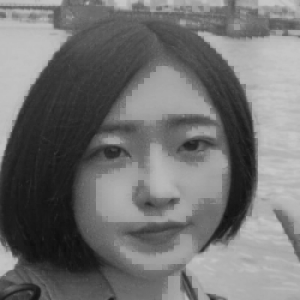
\includegraphics[width=4cm]{./fig/main7_50.png}
		\caption{入力例7(配置II)}
		\label{fig:m7_50}
    \end{minipage}
	% \url{http://www.this.is.sample.url/} % Web上のデータの場合、参照先URLを明記
\end{figure}
\begin{table}[H]
    \centering
    \caption{入力例6($\ref{fig:exg6}$)と入力例7($\ref{fig:exg7}$)での完成手数}
    \begin{tabular}{|c|c|c|c|} \hline
    　 & $n=20$ & $n=30$ & $n=50$ \\ \hline
    先行研究（再現） & 20,970 & 70,354 & 342,415 \\ \hline
    本研究 & 21,246 & 70,998 & 342,799 \\ \hline
    \end{tabular}
    \label{tab:6_7pzl}
\end{table}
\newpage
\textbf{入力例8と入力例9}

\textbf{n=20}
\begin{figure}[H]
	\centering
	\begin{minipage}[t]{0.3\hsize}
		\centering
		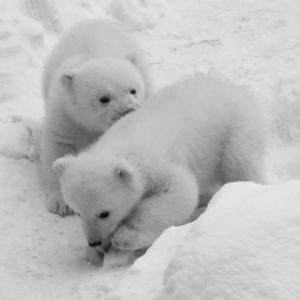
\includegraphics[width=4cm]{./fig/g8.png}
		\caption{入力例8(グレー)}
		\label{fig:exg8}
	\end{minipage}
	\begin{minipage}[t]{0.3\hsize}
		\centering
		
\includegraphics[width=4cm]{./fig/pre9_20.png}
		\caption{入力例9(配置I)}
		\label{fig:p9_20}
    \end{minipage}
	% \url{http://www.this.is.sample.url/} % Web上のデータの場合、参照先URLを明記
\end{figure}
\begin{figure}[H]
	\centering
	\begin{minipage}[t]{0.3\hsize}
		\centering
		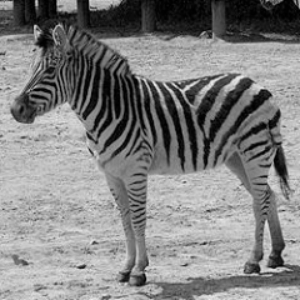
\includegraphics[width=4cm]{./fig/g9.png}
		\caption{入力例9(グレー)}
		\label{fig:exg9}
    \end{minipage}
    \begin{minipage}[t]{0.3\hsize}
		\centering
		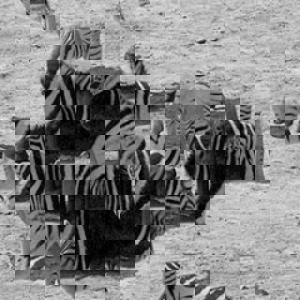
\includegraphics[width=4cm]{./fig/pre8_20.png}
        \caption{入力例8(配置I)}
		\label{fig:p8_20}
    \end{minipage}
	% \url{http://www.this.is.sample.url/} % Web上のデータの場合、参照先URLを明記
\end{figure}
\begin{figure}[H]
	\centering
	\begin{minipage}[t]{0.3\hsize}
		\centering
		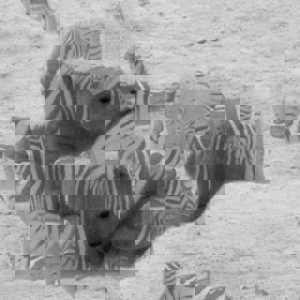
\includegraphics[width=4cm]{./fig/main8_20.png}
        \caption{入力例8(配置II)}
		\label{fig:m8_20}
    \end{minipage}
    \begin{minipage}[t]{0.3\hsize}
		\centering
		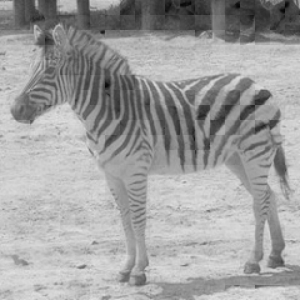
\includegraphics[width=4cm]{./fig/main9_20.png}
		\caption{入力例9(配置II)}
		\label{fig:m9_20}
    \end{minipage}
	% \url{http://www.this.is.sample.url/} % Web上のデータの場合、参照先URLを明記
\end{figure}
\newpage
\textbf{n=30}
\begin{figure}[H]
	\centering
	\begin{minipage}[t]{0.3\hsize}
		\centering
		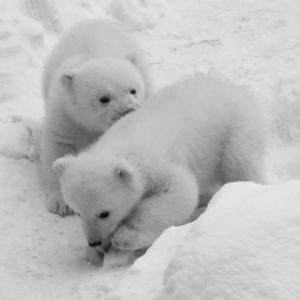
\includegraphics[width=4cm]{./fig/g8.png}
		\caption{入力例8(グレー)}
		\label{fig:exg8}
	\end{minipage}
	\begin{minipage}[t]{0.3\hsize}
		\centering
		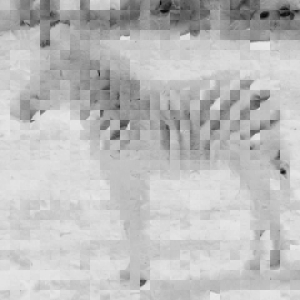
\includegraphics[width=4cm]{./fig/pre9_30.png}
		\caption{入力例9(配置I)}
		\label{fig:p9_30}
    \end{minipage}
	% \url{http://www.this.is.sample.url/} % Web上のデータの場合、参照先URLを明記
\end{figure}
\begin{figure}[H]
	\centering
	\begin{minipage}[t]{0.3\hsize}
		\centering
		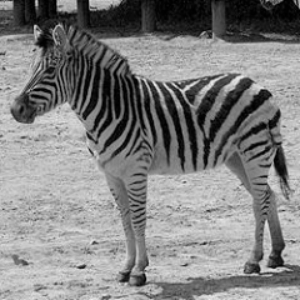
\includegraphics[width=4cm]{./fig/g9.png}
		\caption{入力例9(グレー)}
		\label{fig:exg9}
    \end{minipage}
    \begin{minipage}[t]{0.3\hsize}
		\centering
		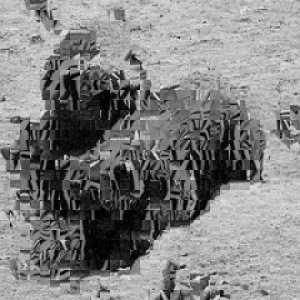
\includegraphics[width=4cm]{./fig/pre8_30.png}
        \caption{入力例8(配置I)}
		\label{fig:p8_30}
    \end{minipage}
	% \url{http://www.this.is.sample.url/} % Web上のデータの場合、参照先URLを明記
\end{figure}
\begin{figure}[H]
	\centering
	\begin{minipage}[t]{0.3\hsize}
		\centering
		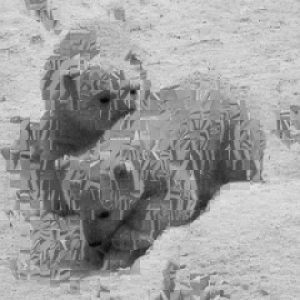
\includegraphics[width=4cm]{./fig/main8_30.png}
        \caption{入力例8(配置II)}
		\label{fig:m8_30}
    \end{minipage}
    \begin{minipage}[t]{0.3\hsize}
		\centering
		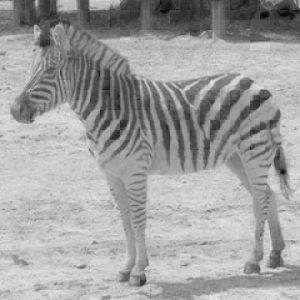
\includegraphics[width=4cm]{./fig/main9_30.png}
		\caption{入力例9(配置II)}
		\label{fig:m9_30}
    \end{minipage}
	% \url{http://www.this.is.sample.url/} % Web上のデータの場合、参照先URLを明記
\end{figure}
\newpage
\textbf{n=50}
\begin{figure}[H]
	\centering
	\begin{minipage}[t]{0.3\hsize}
		\centering
		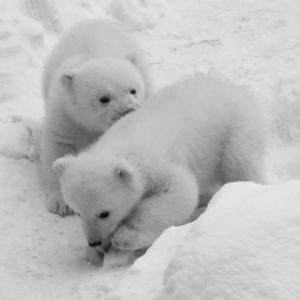
\includegraphics[width=4cm]{./fig/g8.png}
		\caption{入力例8(グレー)}
		\label{fig:exg8}
	\end{minipage}
	\begin{minipage}[t]{0.3\hsize}
		\centering
		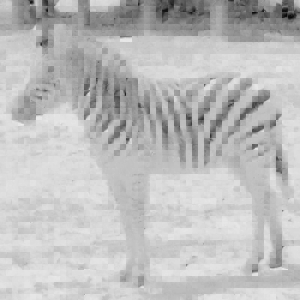
\includegraphics[width=4cm]{./fig/pre9_50.png}
		\caption{入力例9(配置I)}
		\label{fig:p9_50}
    \end{minipage}
	% \url{http://www.this.is.sample.url/} % Web上のデータの場合、参照先URLを明記
\end{figure}
\begin{figure}[H]
	\centering
	\begin{minipage}[t]{0.3\hsize}
		\centering
		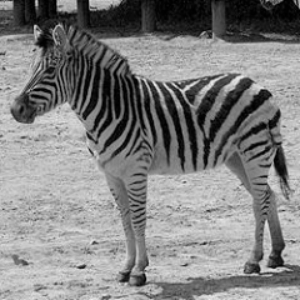
\includegraphics[width=4cm]{./fig/g9.png}
		\caption{入力例9(グレー)}
		\label{fig:exg9}
    \end{minipage}
    \begin{minipage}[t]{0.3\hsize}
		\centering
		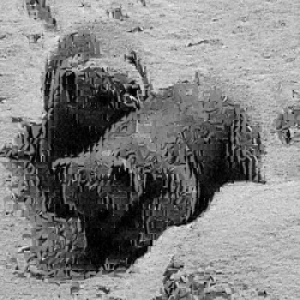
\includegraphics[width=4cm]{./fig/pre8_50.png}
        \caption{入力例8(配置I)}
		\label{fig:p8_50}
    \end{minipage}
	% \url{http://www.this.is.sample.url/} % Web上のデータの場合、参照先URLを明記
\end{figure}
\begin{figure}[H]
	\centering
	\begin{minipage}[t]{0.3\hsize}
		\centering
		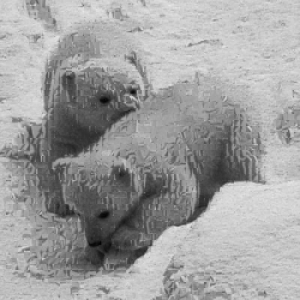
\includegraphics[width=4cm]{./fig/main8_50.png}
        \caption{入力例8(配置II)}
		\label{fig:m8_50}
    \end{minipage}
    \begin{minipage}[t]{0.3\hsize}
		\centering
		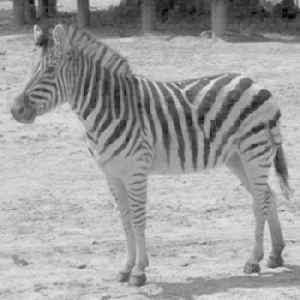
\includegraphics[width=4cm]{./fig/main9_50.png}
		\caption{入力例9(配置II)}
		\label{fig:m9_50}
    \end{minipage}
	% \url{http://www.this.is.sample.url/} % Web上のデータの場合、参照先URLを明記
\end{figure}
\begin{table}[H]
    \centering
    \caption{入力例8($\ref{fig:exg8}$)と入力例9($\ref{fig:exg9}$)での完成手数}
    \begin{tabular}{|c|c|c|c|} \hline
    　 & $n=20$ & $n=30$ & $n=50$ \\ \hline
    先行研究（再現） & 21,731 & 73,753 & 345,281 \\ \hline
    本研究 & 21,329 & 72,449 & 341,595 \\ \hline
    \end{tabular}
    \label{tab:8_9pzl}
\end{table}
\newpage
\textbf{入力例3と入力例10}

\textbf{n=20}
\begin{figure}[H]
	\centering
	\begin{minipage}[t]{0.3\hsize}
		\centering
		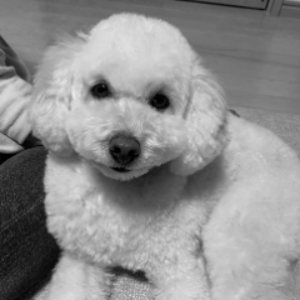
\includegraphics[width=4cm]{./fig/g3.png}
		\caption{入力例3(グレー)}
		\label{fig:exg3}
	\end{minipage}
	\begin{minipage}[t]{0.3\hsize}
		\centering
		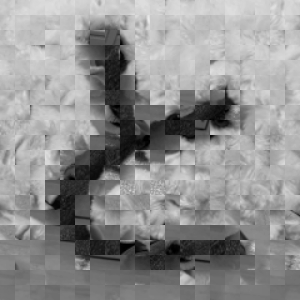
\includegraphics[width=4cm]{./fig/pre10_20.png}
		\caption{入力例10(配置I)}
		\label{fig:p10_20}
    \end{minipage}
    
	% \url{http://www.this.is.sample.url/} % Web上のデータの場合、参照先URLを明記
\end{figure}
\begin{figure}[H]
	\centering
	\begin{minipage}[t]{0.3\hsize}
		\centering
		
\includegraphics[width=4cm]{./fig/g10.png}
		\caption{入力例10(グレー)}
		\label{fig:exg10}
    \end{minipage}
	\begin{minipage}[t]{0.3\hsize}
		\centering
		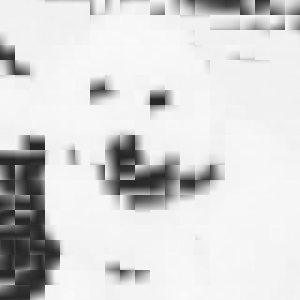
\includegraphics[width=4cm]{./fig/pre3_20.png}
        \caption{入力例3(配置I)}
		\label{fig:p3_20}
    \end{minipage}
	% \url{http://www.this.is.sample.url/} % Web上のデータの場合、参照先URLを明記
\end{figure}
\begin{figure}[H]
	\centering
	\begin{minipage}[t]{0.3\hsize}
		\centering
		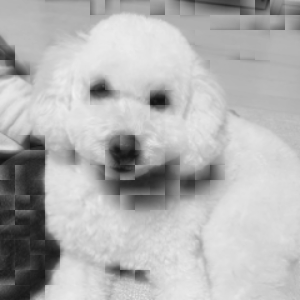
\includegraphics[width=4cm]{./fig/main3_20.png}
        \caption{入力例3(配置II)}
		\label{fig:m3_20}
    \end{minipage}
    \begin{minipage}[t]{0.3\hsize}
		\centering
		
\includegraphics[width=4cm]{./fig/main10_20.png}
		\caption{入力例10(配置II)}
		\label{fig:m10_20}
    \end{minipage}
	% \url{http://www.this.is.sample.url/} % Web上のデータの場合、参照先URLを明記
\end{figure}
\newpage
\textbf{n=30}
\begin{figure}[H]
	\centering
	\begin{minipage}[t]{0.3\hsize}
		\centering
		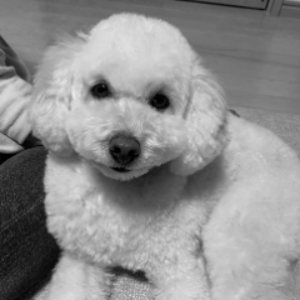
\includegraphics[width=4cm]{./fig/g3.png}
		\caption{入力例3(グレー)}
		\label{fig:exg3}
	\end{minipage}
	\begin{minipage}[t]{0.3\hsize}
		\centering
		
\includegraphics[width=4cm]{./fig/pre10_30.png}
		\caption{入力例10(配置I)}
		\label{fig:p10_30}
    \end{minipage}
    
	% \url{http://www.this.is.sample.url/} % Web上のデータの場合、参照先URLを明記
\end{figure}
\begin{figure}[H]
	\centering
	\begin{minipage}[t]{0.3\hsize}
		\centering
		
\includegraphics[width=4cm]{./fig/g10.png}
		\caption{入力例10(グレー)}
		\label{fig:exg10}
    \end{minipage}
	\begin{minipage}[t]{0.3\hsize}
		\centering
		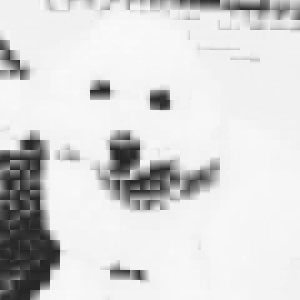
\includegraphics[width=4cm]{./fig/pre3_30.png}
        \caption{入力例3(配置I)}
		\label{fig:p3_30}
    \end{minipage}
	% \url{http://www.this.is.sample.url/} % Web上のデータの場合、参照先URLを明記
\end{figure}
\begin{figure}[H]
	\centering
	\begin{minipage}[t]{0.3\hsize}
		\centering
		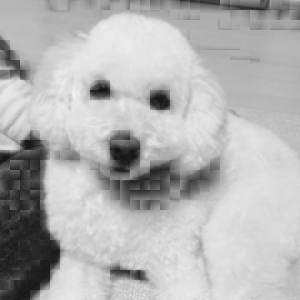
\includegraphics[width=4cm]{./fig/main3_30.png}
        \caption{入力例3(配置II)}
		\label{fig:m3_30}
    \end{minipage}
    \begin{minipage}[t]{0.3\hsize}
		\centering
		
\includegraphics[width=4cm]{./fig/main10_30.png}
		\caption{入力例10(配置II)}
		\label{fig:m10_30}
    \end{minipage}
	% \url{http://www.this.is.sample.url/} % Web上のデータの場合、参照先URLを明記
\end{figure}
\newpage
\textbf{n=50}
\begin{figure}[H]
	\centering
	\begin{minipage}[t]{0.3\hsize}
		\centering
		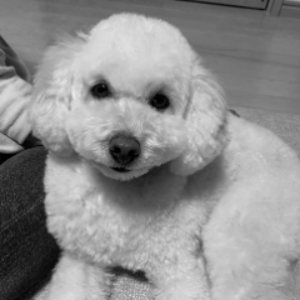
\includegraphics[width=4cm]{./fig/g3.png}
		\caption{入力例3(グレー)}
		\label{fig:exg3}
	\end{minipage}
	\begin{minipage}[t]{0.3\hsize}
		\centering
		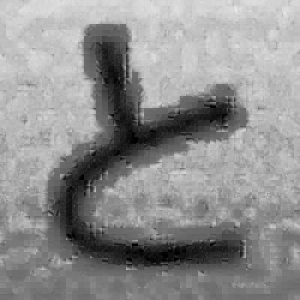
\includegraphics[width=4cm]{./fig/pre10_50.png}
		\caption{入力例10(配置I)}
		\label{fig:p10_50}
    \end{minipage}
	% \url{http://www.this.is.sample.url/} % Web上のデータの場合、参照先URLを明記
\end{figure}
\begin{figure}[H]
	\centering
	\begin{minipage}[t]{0.3\hsize}
		\centering
		
\includegraphics[width=4cm]{./fig/g10.png}
		\caption{入力例10(グレー)}
		\label{fig:exg10}
    \end{minipage}
	\begin{minipage}[t]{0.3\hsize}
		\centering
		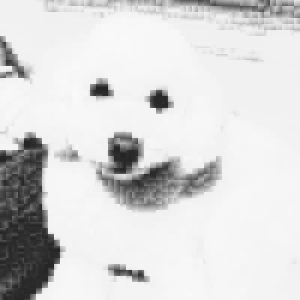
\includegraphics[width=4cm]{./fig/pre3_50.png}
        \caption{入力例3(配置I)}
		\label{fig:p3_50}
    \end{minipage}
	% \url{http://www.this.is.sample.url/} % Web上のデータの場合、参照先URLを明記
\end{figure}
\begin{figure}[H]
	\centering
	\begin{minipage}[t]{0.3\hsize}
		\centering
		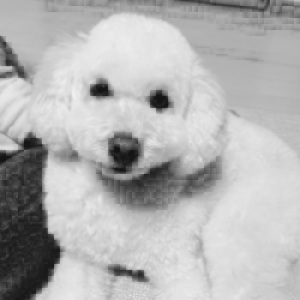
\includegraphics[width=4cm]{./fig/main3_50.png}
        \caption{入力例3(配置II)}
		\label{fig:m3_50}
    \end{minipage}
    \begin{minipage}[t]{0.3\hsize}
		\centering
		
\includegraphics[width=4cm]{./fig/main10_50.png}
		\caption{入力例10(配置II)}
		\label{fig:m10_50}
    \end{minipage}
	% \url{http://www.this.is.sample.url/} % Web上のデータの場合、参照先URLを明記
\end{figure}
\begin{table}[H]
    \centering
    \caption{入力例3($\ref{fig:exg3}$)と入力例10($\ref{fig:exg10}$)での完成手数}
    \begin{tabular}{|c|c|c|c|} \hline
    　 & $n=20$ & $n=30$ & $n=50$ \\ \hline
    先行研究（再現） & 20,382 & 70,327 & 335,377 \\ \hline
    本研究 & 20,638 & 70,355 & 330,369 \\ \hline
    \end{tabular}
    \label{tab:3_10pzl}
\end{table}
\newpage

以下は，$n=20,30,50$において，全ての組み合わせの手数をまとめたものである．マスの上部が先行研究の再現による手数で，下部が本研究による手数である．
\begin{figure}[H]
    \centering
    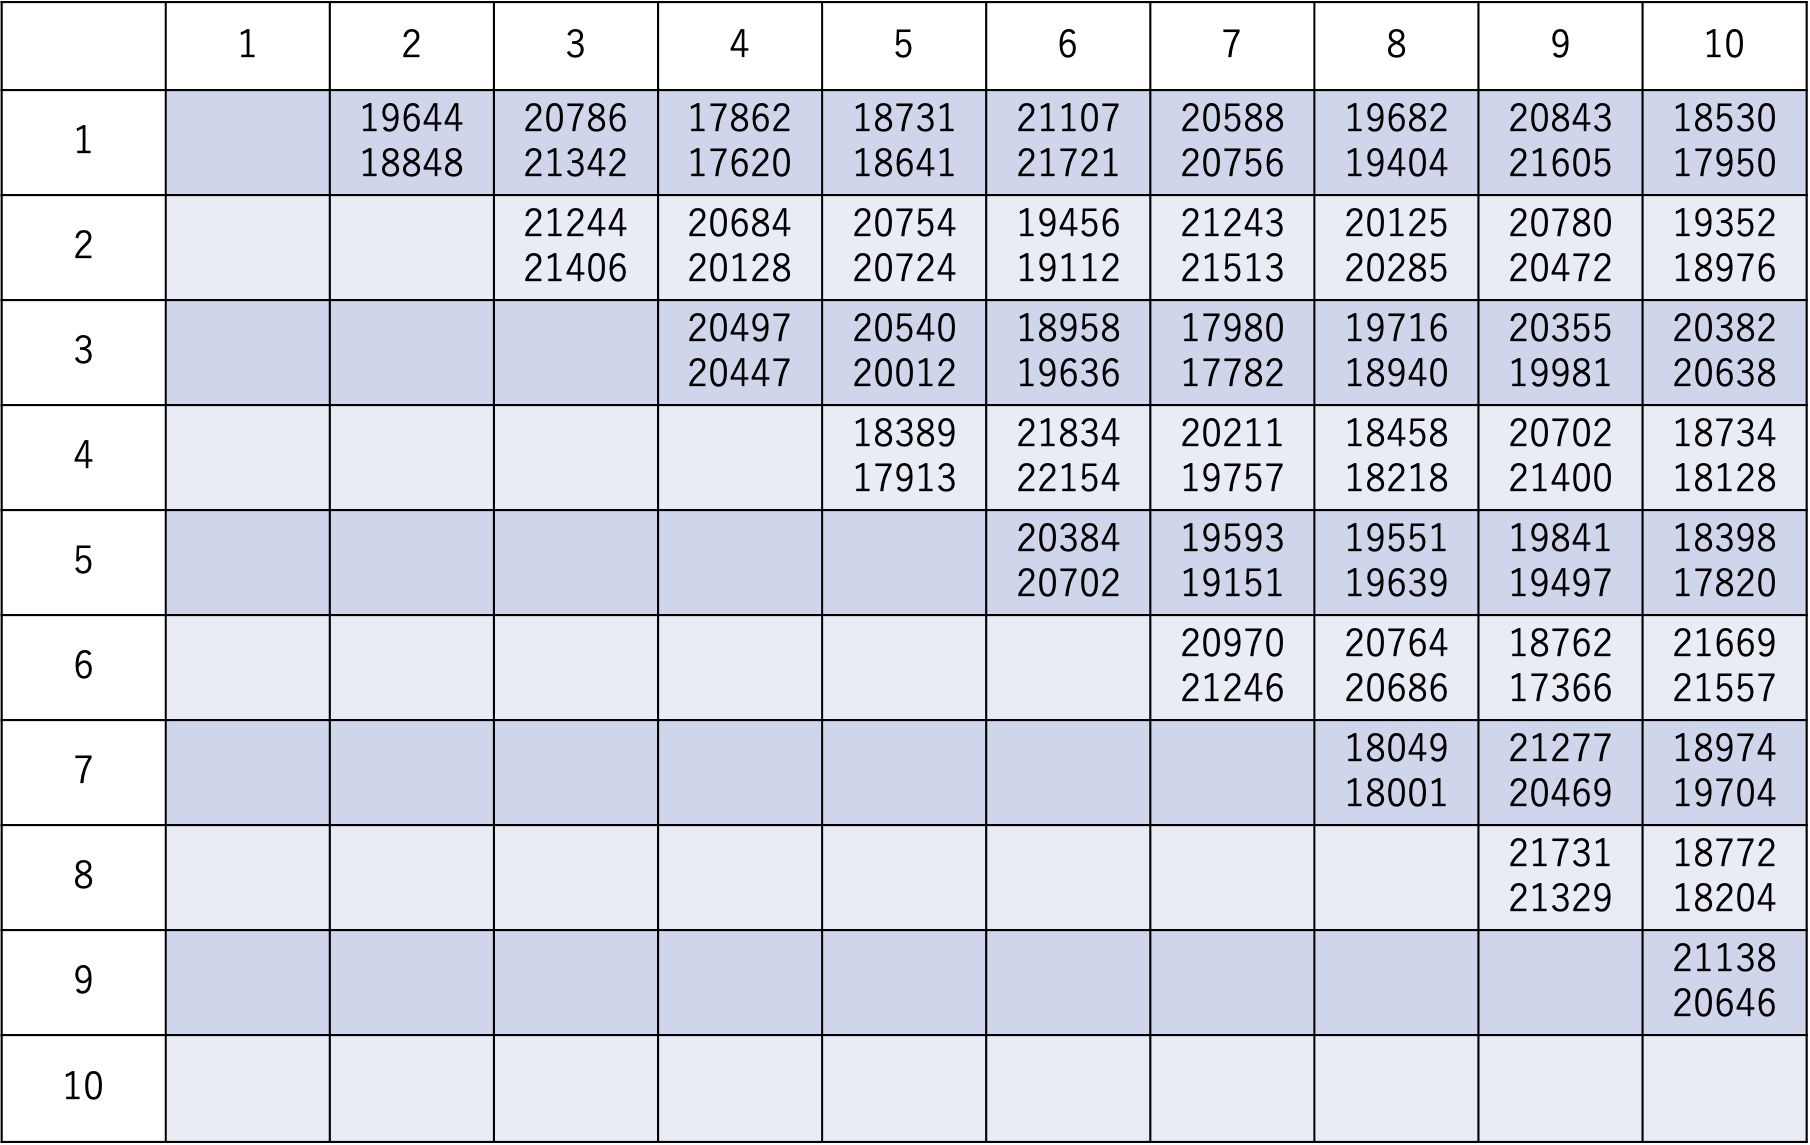
\includegraphics[width=10cm]{./fig/n20.png}
    \caption{n=20の手数}
    \label{fig:n20}
	% \url{http://www.this.is.sample.url/} % Web上のデータの場合、参照先URLを明記
\end{figure}
\begin{figure}[H]
    \centering
    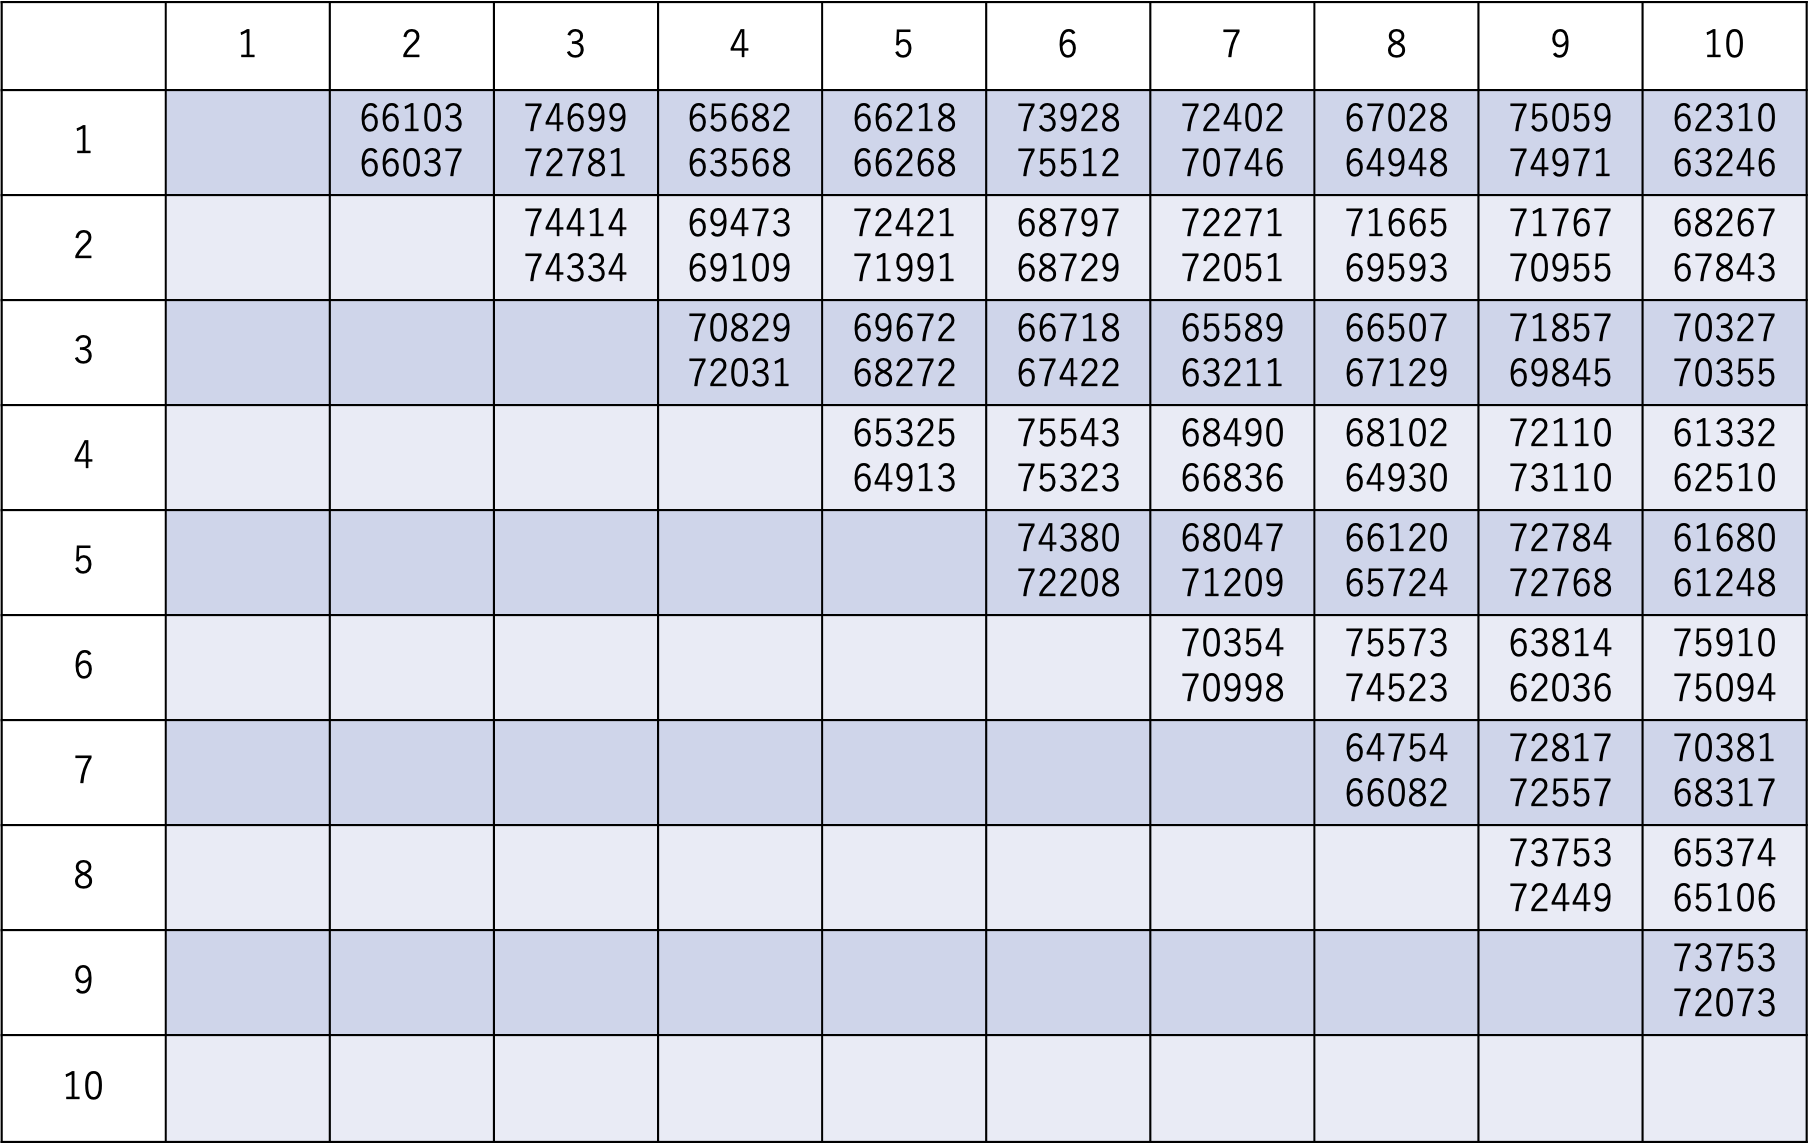
\includegraphics[width=10cm]{./fig/n30.png}
    \caption{n=30の手数}
    \label{fig:n30}
	% \url{http://www.this.is.sample.url/} % Web上のデータの場合、参照先URLを明記
\end{figure}
\begin{figure}[H]
    \centering
    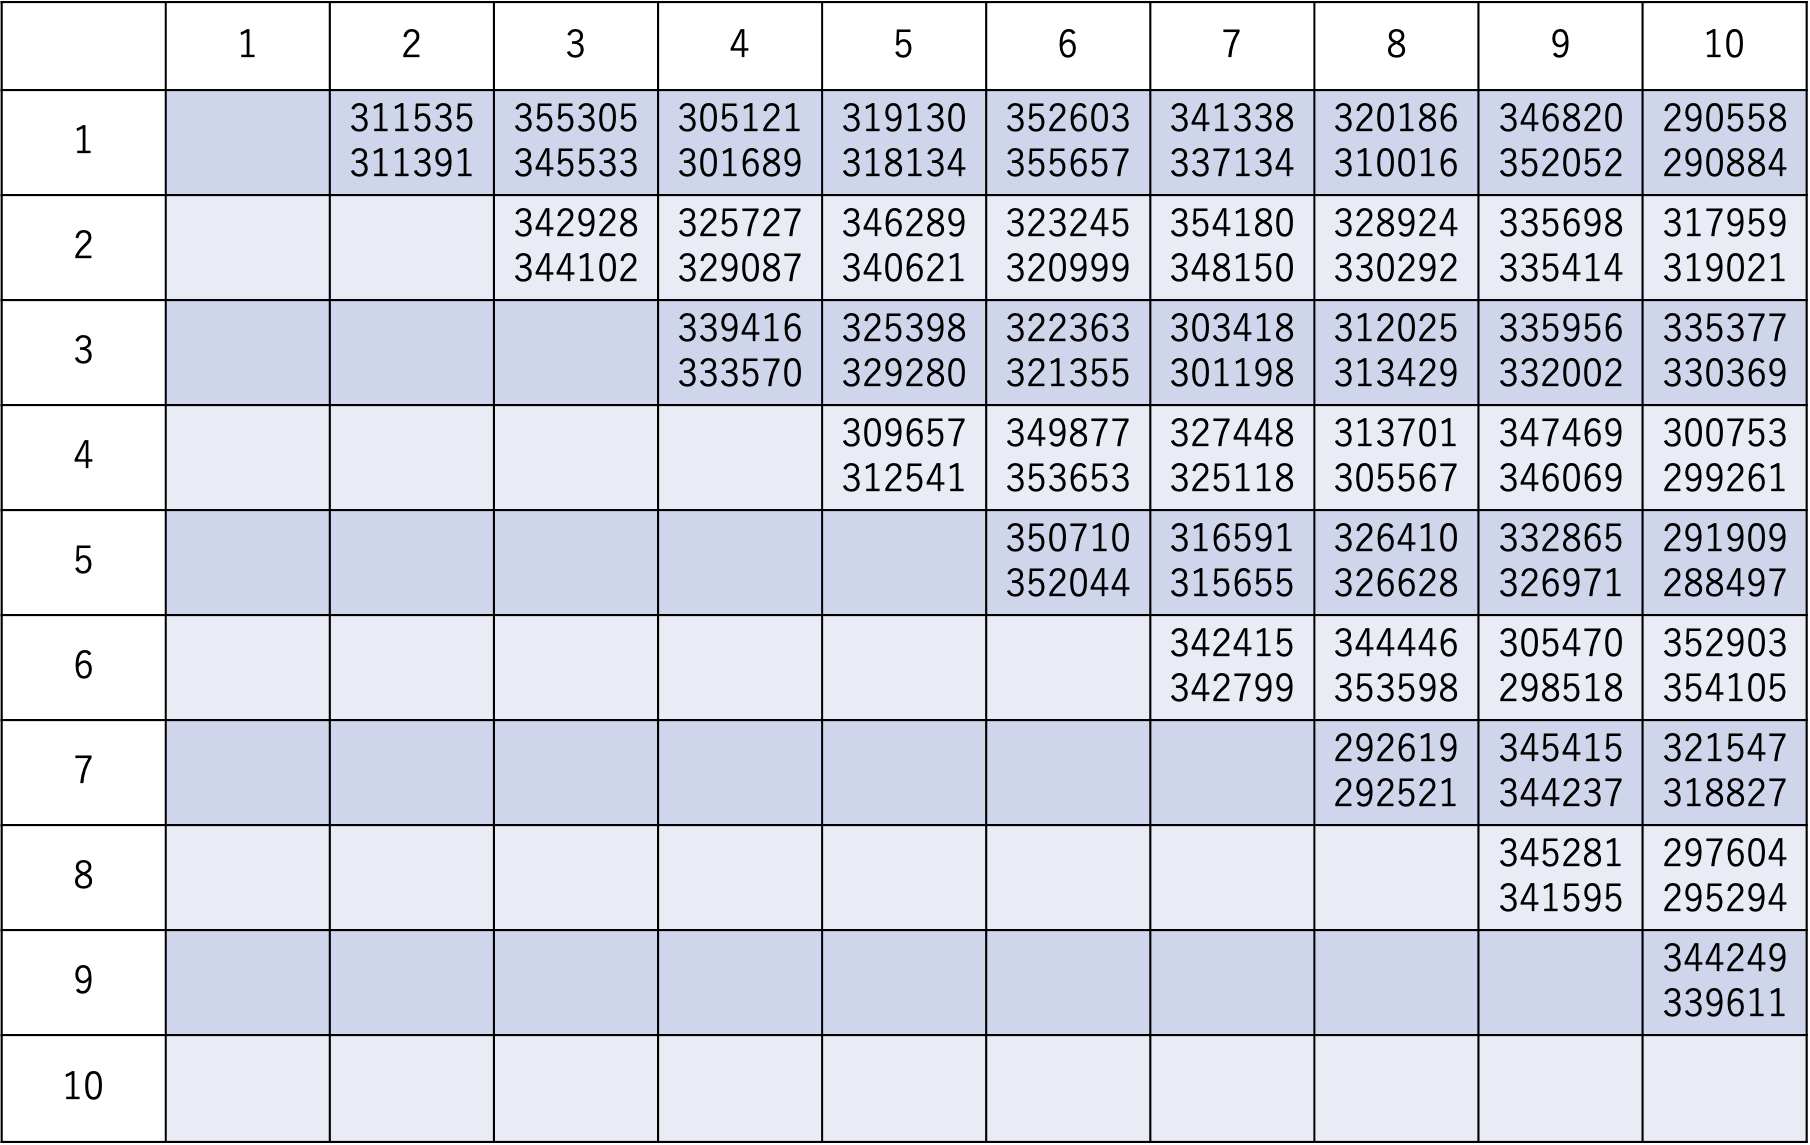
\includegraphics[width=10cm]{./fig/n50.png}
    \caption{n=50の手数}
    \label{fig:n50}
	% \url{http://www.this.is.sample.url/} % Web上のデータの場合、参照先URLを明記
\end{figure}

\begin{table}[H]
    \centering
    \caption{完成手数の平均値(切り捨て)}
    \begin{tabular}{|c|c|c|c|} \hline
    　 & $n=20$ & $n=30$ & $n=50$ \\ \hline
    先行研究（再現） & 19,956 & 69,653 & 327,796 \\ \hline
    本研究 & 19,811 & 69,132 & 326,321 \\ \hline
    先行研究 & × & 75,214 & 346,890 \\ \hline
    \end{tabular}
    \label{tab:avepzl}
\end{table}
